\title{Midterm 2 for COSC330/PHYS306 - Fall 2021}
\author{Dr. Jordan Hanson - Whittier College Dept. of Physics and Astronomy}
\date{\today}
\documentclass[10pt]{article}
\usepackage[a4paper, total={18cm, 27cm}]{geometry}
\usepackage{outlines}
\usepackage{graphicx}
\begin{document}
\maketitle

\section{Chapter 6 - Functions of Combinational Logic}
\label{sec:comb2}

\begin{enumerate}
\item Consider Fig. \ref{fig:4bit_wDelay}, in which a 4-bit adder is depicted.  Assuming a uniform worst-case delay of 8 ns from carry-in to carry-out for each stage, the total delay is 32 ns.  (a) At what maximum frequency can this circuit perform additions, if the delay must be less than a clock period? (b) What would the result in (a) be if the adder was extended to 8 bits? (c) Create a timing diagram showing the addition of the numbers in Fig. \ref{fig:4bit_wDelay}. \textbf{Bonus:} include the timing delays, and indicate the clock period.
\begin{figure}[ht]
\centering
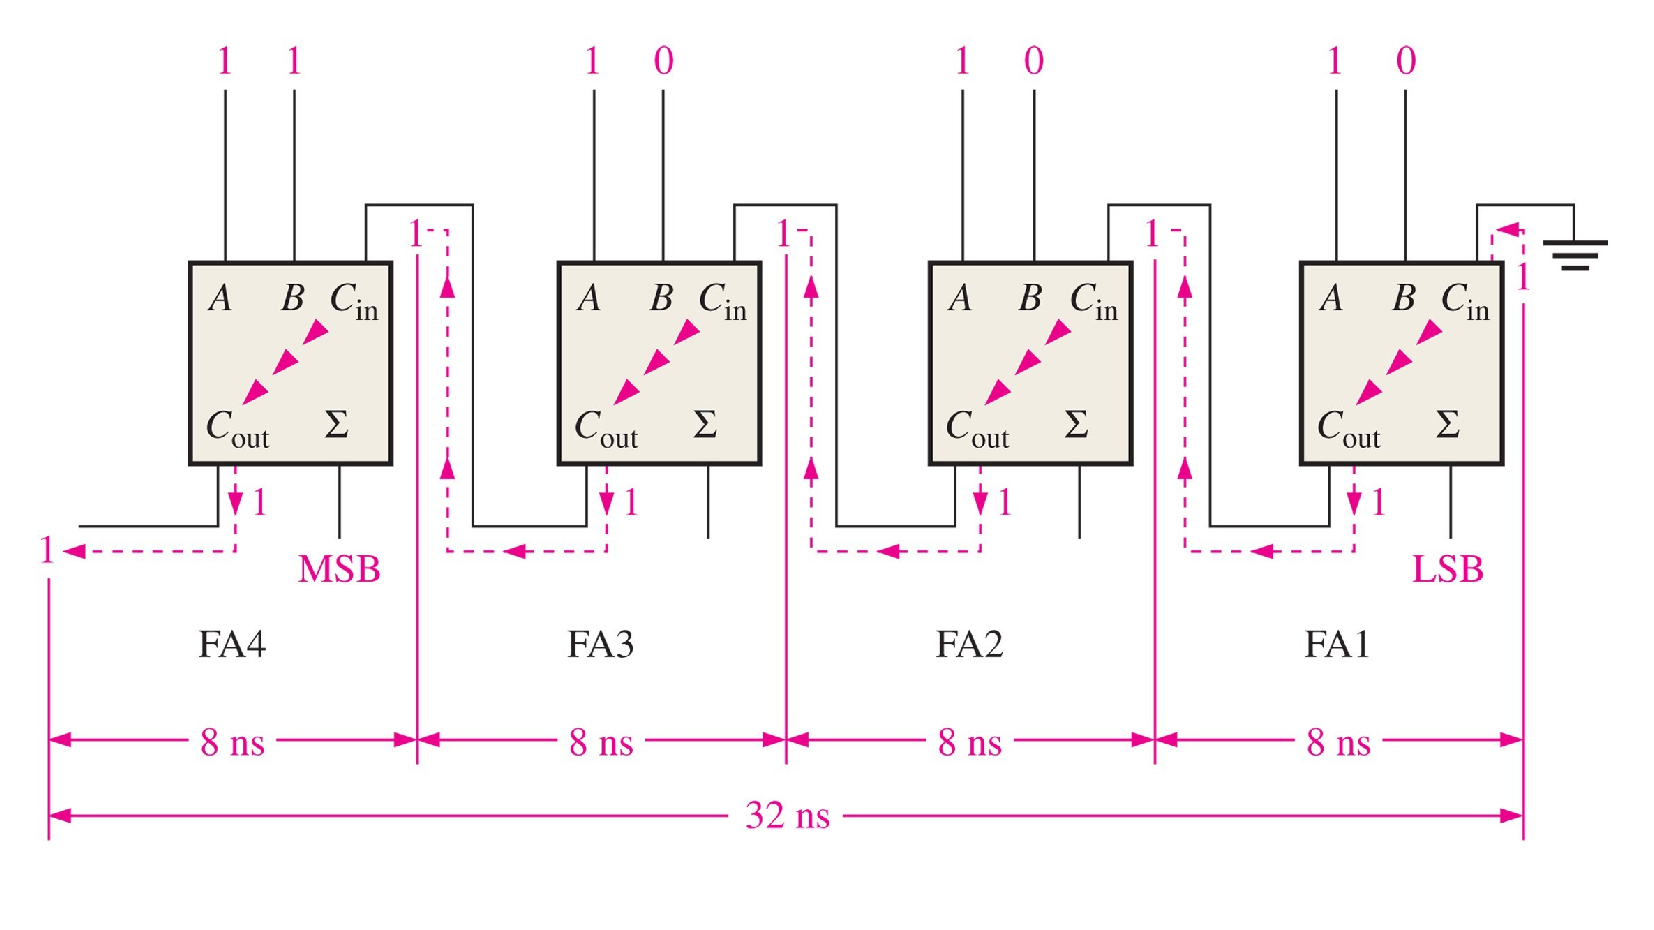
\includegraphics[width=0.75\textwidth]{figures/4bitadder_withDelay.pdf}
\caption{\label{fig:4bit_wDelay} A schematic of a 4-bit adder with delays marked in nanoseconds.}
\end{figure}
\item Using AND, OR, XNOR, and inverter gates, (a) create a 2-bit comparator that yields True if $A > B$, (b) True if $A = B$, and (c) True if $A < B$.  For each circuit, assume both $A$ and $B$ are 2-bit binary positive numbers. (d) Wrap this all into one circuit with three outputs and 4 inputs.  \textit{Hint: use Karnaugh maps for parts (a)-(c) to simplify the gates.} \\ \vspace{3.5cm}
\item Generate the logic gates that convert 4-bit gray code to 4-bit binary code, and show that it works with a timing diagram. \\ \vspace{3cm}
\item Consider Fig. \ref{fig:enc}, in which a decimal to binary conversion circuit is shown. (a) Add logic to the circuit such that it becomes a hexadecimal to binary converter. (b) Draw a logic symbol for this circuit with the correct number of inputs and outputs.  (c) Connect two hex-to-bin converters to a symbolic 2-to-1 multiplexer with the correct number of data select line(s) to form a system that can send two-digit hex numbers over one output line.
\begin{figure}[ht]
\centering
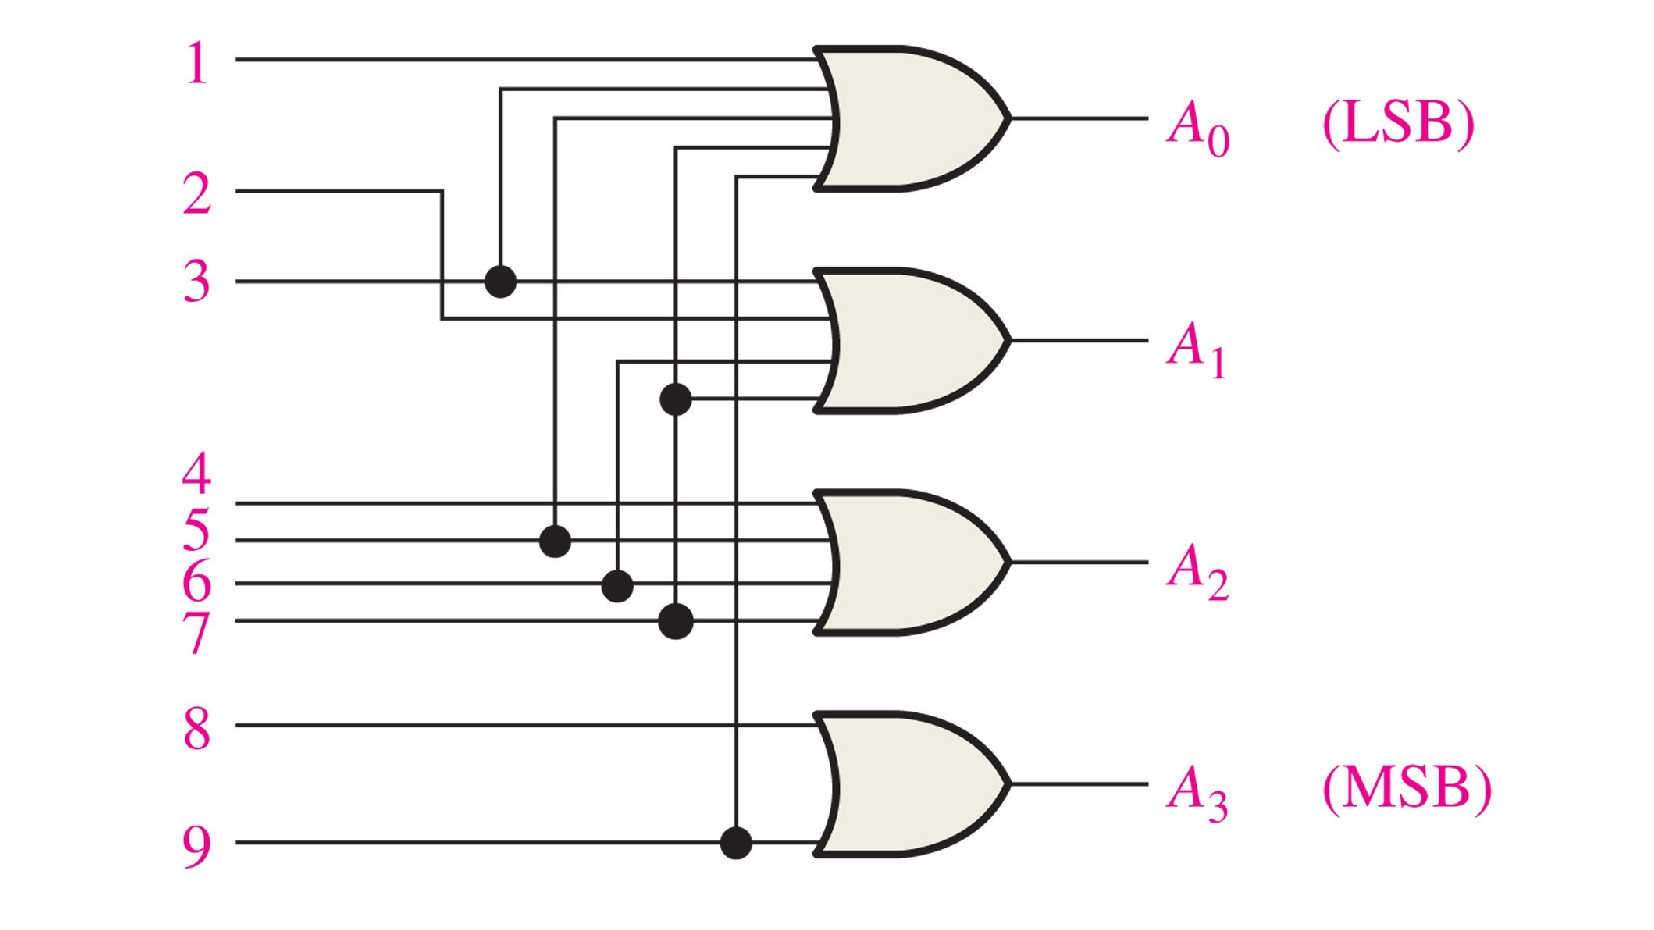
\includegraphics[width=0.5\textwidth]{figures/encoder.pdf}
\caption{\label{fig:enc} A decimal to binary encoder circuit.}
\end{figure} \vspace{2cm}
\end{enumerate}

\section{Chapter 7 - Latches, Flip-flops, and Timers}
\label{sec:latch}
\begin{enumerate}
\item Consider Fig. \ref{fig:twoDFF}, in which a divide-by-four frequency divider is depicted with D flip-flops and a CLK signal. (a) Elaborate on this circuit to create a circuit that can divide the clock frequency by 2, 4, or 8. Show the flip-flops explicitly.  (b) Develop a symbol for the 2-4-8-16 divider, with CLK signal input and four ouputs (one each for $f/2$, $f/4$, $f/8$, and $f/8$, where $f$ is the clock frequency). (c) Connect the symbol for the new part to a symbolic 4-to-1 multiplexer with the appropriate number of data select lines to form a clock division system.  (d) Show with a timing diagram the output if the user changes the data select lines at least once.  For parts (b)-(d), it is only necessary to show symbols rather than individual flip-flops.
\begin{figure}[ht]
\centering
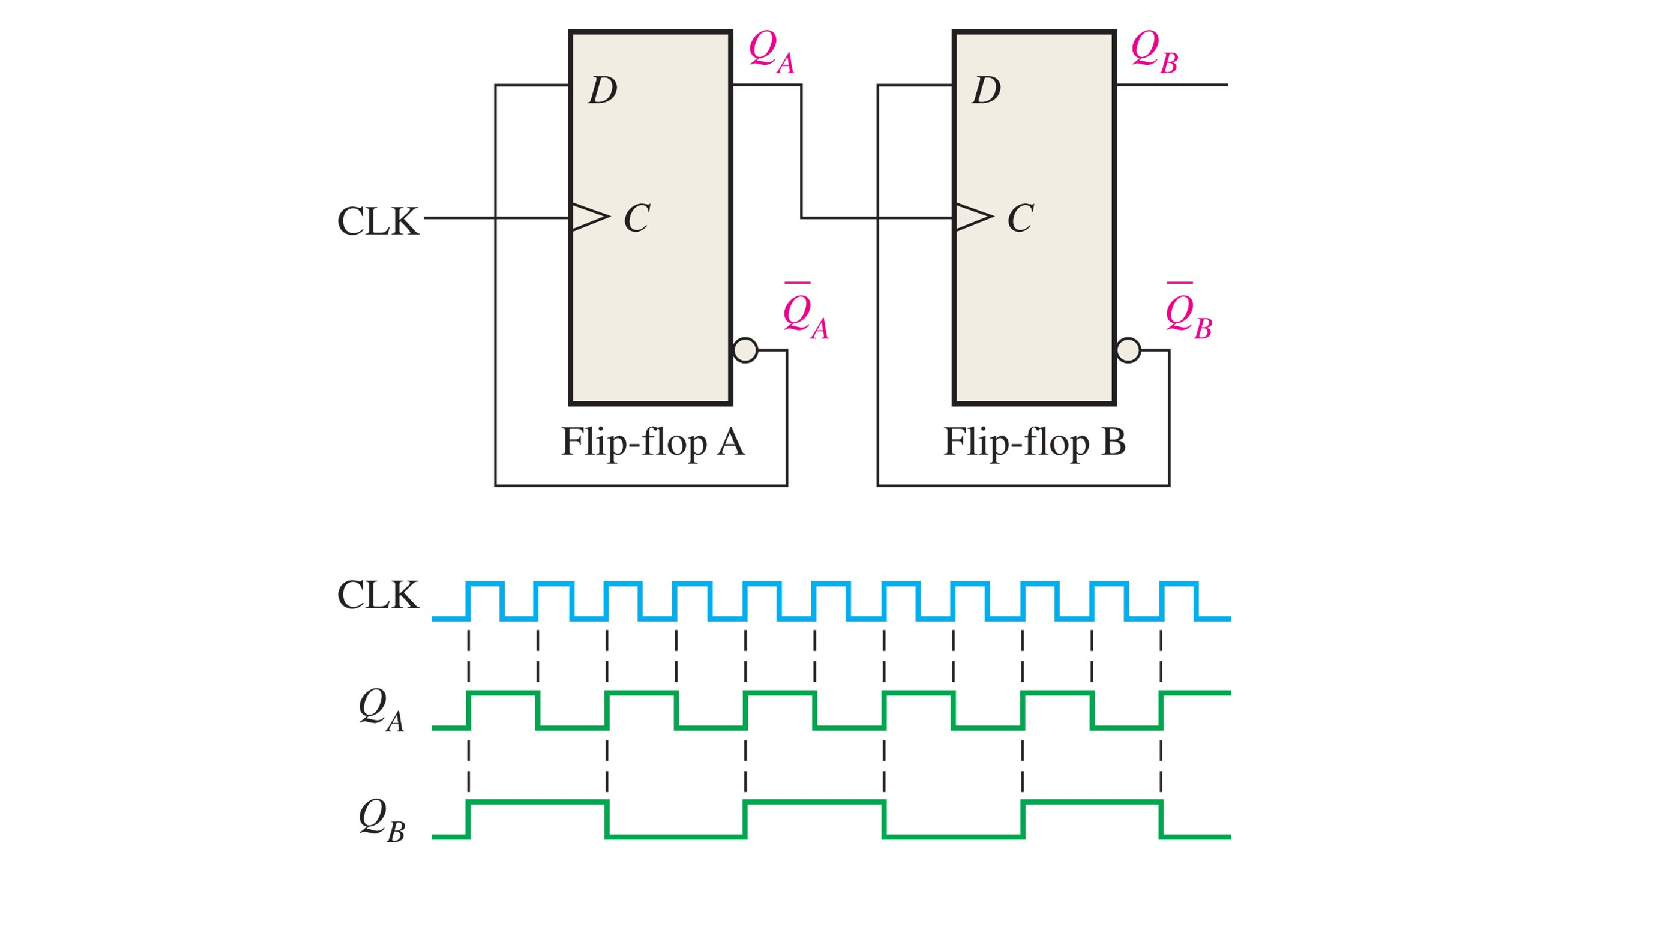
\includegraphics[width=0.55\textwidth]{figures/twoDFF.pdf}
\caption{\label{fig:twoDFF} Two D flip-flops forming a frequency divider.}
\end{figure}
\end{enumerate}

\clearpage

\section{Chapters 8 and 9 - Shift Registers and Counters}

\begin{enumerate}
\item Consider the timing diagram in Fig. \ref{fig:sr1}.  Using any combination of \textit{shift registers} and supporting gates, create a circuit with 8-outputs that produces this timing diagram.
\begin{figure}[ht]
\centering
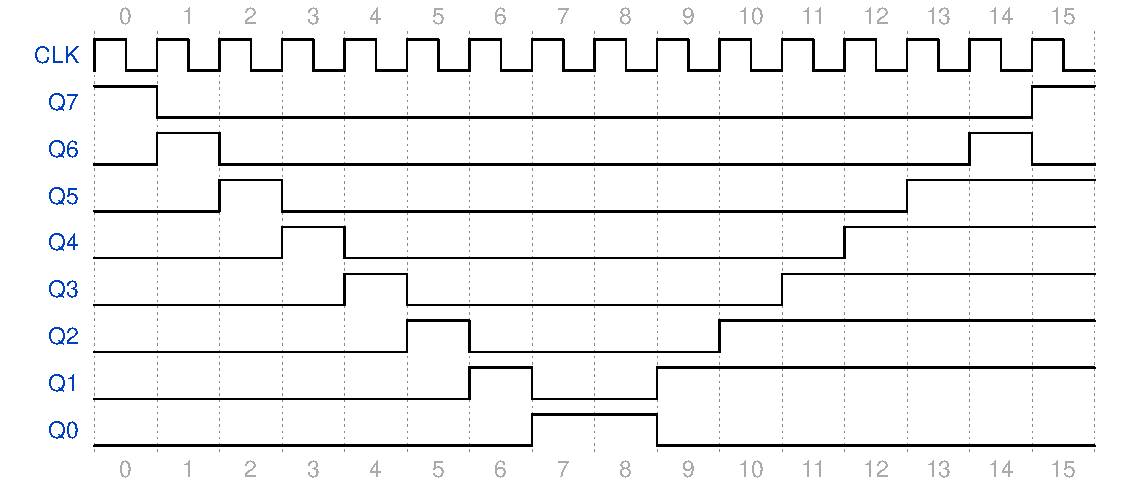
\includegraphics[width=0.5\textwidth]{figures/timingExample15.pdf}
\caption{\label{fig:sr1} A waveform that repeats every 16 clock periods.}
\end{figure} \vspace{4cm}
\item Consider Fig. \ref{fig:SRG8}, in which 4 and 5-bit Johnson counters are depicted.  (a) Create a circuit based on Fig. \ref{fig:SRG8} called a \textit{combinatoric trigger.}  Imagine four digital channels A, B, C, and D, as inputs.  The output of the circuit should be True if \textit{any two} of the four channels is True \textit{within 100 ns of each other.}  Develop any necessary logic symbols, and use the appropriate clock frequency.  The Johnson counter(s) can have any number of bits.
\begin{figure}[hb]
\centering
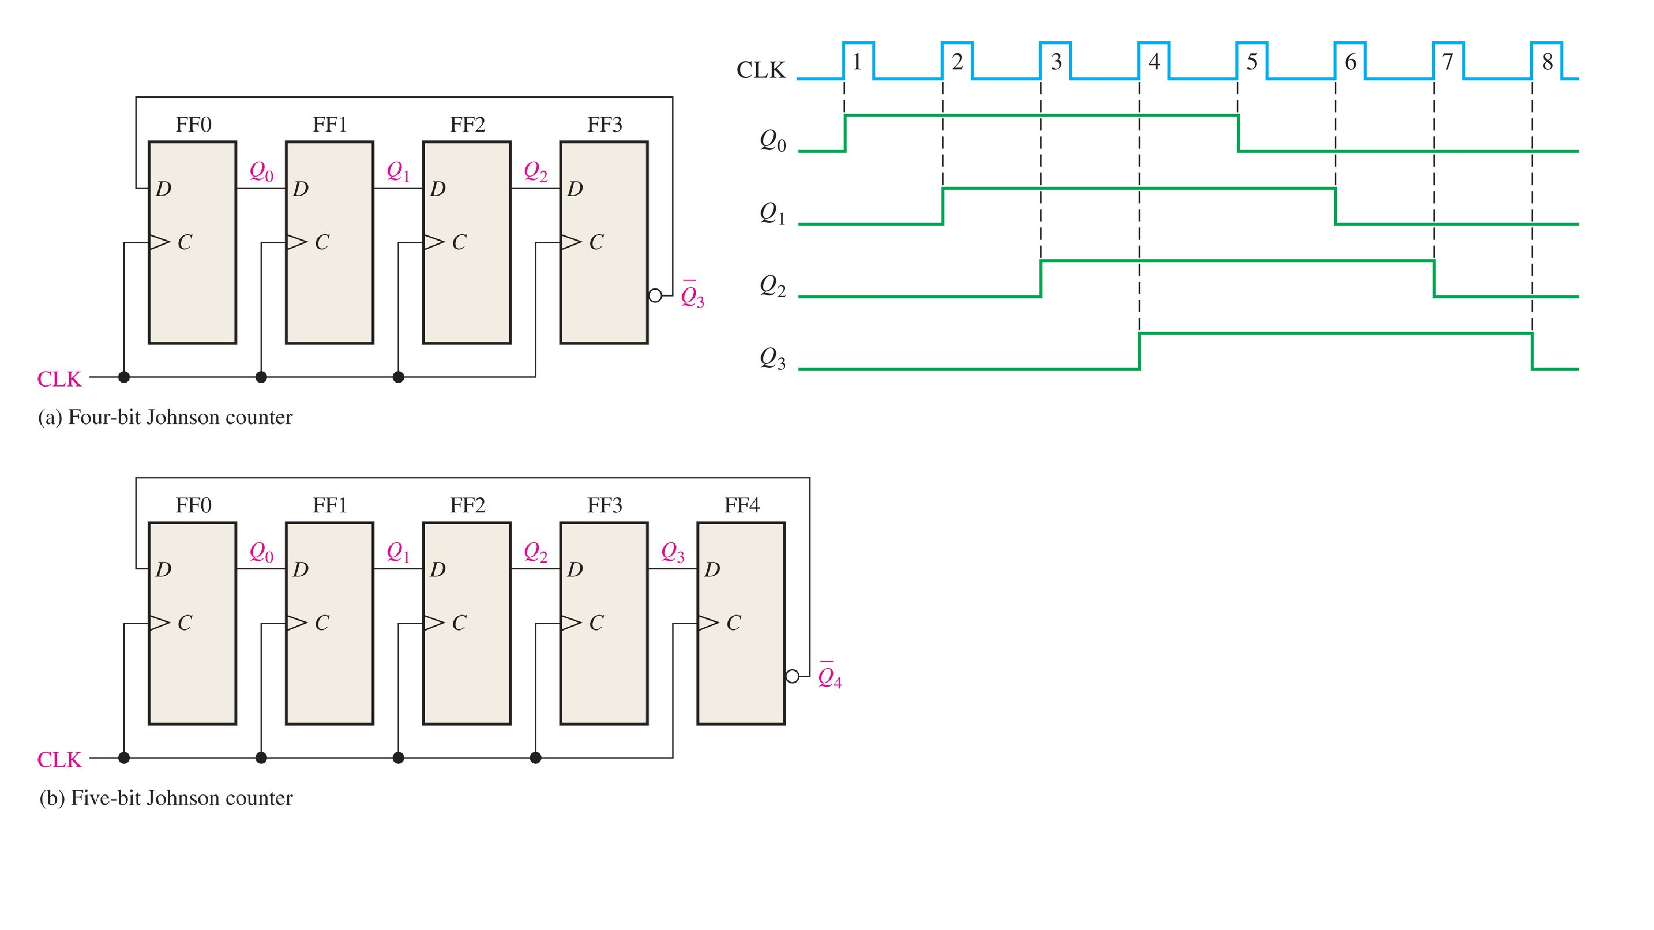
\includegraphics[width=0.8\textwidth]{figures/SRG8.pdf}
\caption{\label{fig:SRG8} (Left) 4 and 5-bit Johnson counters. (Right) The timing diagram for the 4-bit case.}
\end{figure}
\end{enumerate}

\end{document}